\documentclass[tikz,border=6pt]{standalone}
\usepackage{pgfplots}
\pgfplotsset{compat=1.18}

\begin{document}
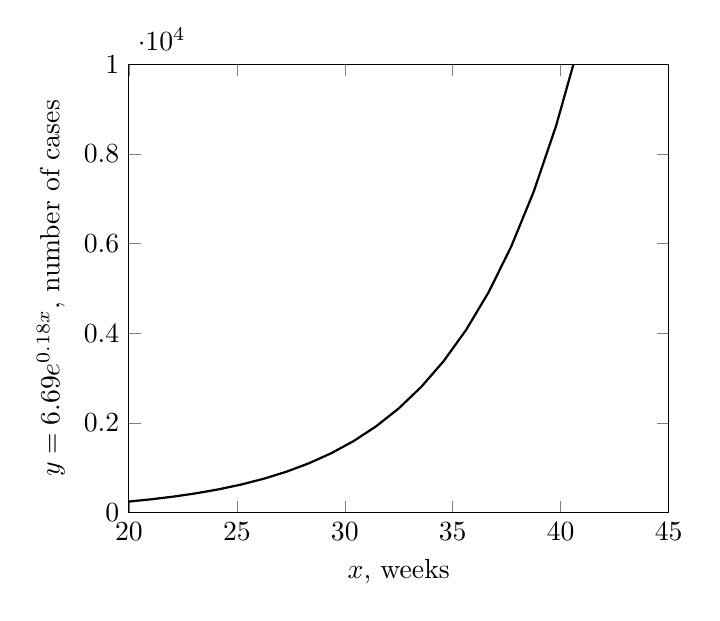
\begin{tikzpicture}
\begin{axis}[
    xlabel={$x$, weeks},
    ylabel={$y = 6.69e^{0.18x}$, number of cases},
    xmin=20, xmax=45,
    ymin=0, ymax=10000,
]
    % Gráfica de y = e^x
    \addplot[domain=20:45, thick] {6.69*exp(0.18*x)};
\end{axis}
\end{tikzpicture}
\end{document}